\documentclass[10pt,aspectratio=169,serif,fleqn]{beamer}

\usepackage[fontset=none, scheme=plain]{ctex}
\IfFontExistsTF{Songti SC}{%
	\setCJKmainfont{Songti SC}[AutoFakeSlant=0.2]%
	\setCJKsansfont{Songti SC}[AutoFakeSlant=0.2]%
}{%
	\setCJKmainfont{FandolSong-Regular}[Extension=.otf,BoldFont=FandolSong-Bold,AutoFakeSlant=0.2]%
	\setCJKsansfont{FandolSong-Regular}[Extension=.otf,BoldFont=FandolSong-Bold]%
}
\usepackage{amsmath,amssymb,graphicx,tikz,booktabs,multicol,calligra}
\usepackage{pgfplots}
\pgfplotsset{compat=1.18}
\usepackage{tcolorbox}
\tcbuselibrary{skins}
\usepackage{XyygU}
\usepackage{caption}
\captionsetup[figure]{name=图,labelsep=period}

\usetikzlibrary{arrows.meta,positioning,calc}

\setlength{\abovedisplayskip}{0pt plus 2pt minus 2pt}
\setlength{\belowdisplayskip}{0pt plus 2pt minus 2pt}

\title[习题4.2]{习题4.2 指数函数}
\subtitle{定义域 \,$\cdot$\, 单调性 \,$\cdot$\, 指数模型}
\author{}
\institute{}
\date{2026-10-16}

\begin{document}

\begin{frame}
  \titlepage
\end{frame}

% ========== 第1题 ==========
\begin{frame}[t]{第1题：求指数函数的定义域}
\textbf{1.} 求下列函数的定义域：
\[
(1)\ y=2^{3-x};\qquad
(2)\ y=3^{2x+1};\qquad
(3)\ y=\left(\frac{1}{2}\right)^{5x};\qquad
(4)\ y=0.7^{\frac{1}{x}}.
\]
\end{frame}

\begin{frame}[t]{第1题 解答}
\begin{tcolorbox}[colback=orange!10,colframe=orange,title=\textbf{解}]
指数函数 $y=a^{u}$ 对任意实数 $u$ 都有意义，因此只需考虑 $u$ 自身的取值范围。

\[
(1)\ u=3-x\in\mathbf{R},\quad \text{定义域为 }\alert{\mathbf{R}}.
\]
\[
(2)\ u=2x+1\in\mathbf{R},\quad \text{定义域为 }\alert{\mathbf{R}}.
\]
\[
(3)\ u=5x\in\mathbf{R},\quad \text{定义域为 }\alert{\mathbf{R}}.
\]
\[
(4)\ u=\frac{1}{x}\ \text{要求 }x\ne 0,\quad \text{定义域为 }\alert{(-\infty,0)\cup(0,+\infty)}.
\]
\end{tcolorbox}
\end{frame}

% ========== 第2题 ==========
\begin{frame}[t]{第2题：产量增长模型}
\textbf{2.} 一种产品原来的年产量是 $a$ 件，今后 $m$ 年内，计划使产量平均每年比上一年增加 $p\%$，写出年产量 $y$（单位：件）关于经过的年数 $x$ 的函数解析式。
\end{frame}

\begin{frame}[t]{第2题 解答}
\begin{tcolorbox}[colback=orange!10,colframe=orange,title=\textbf{解}]
原产量为 $a$；
\begin{itemize}
  \item $1$ 年后产量为 $a(1+p\%)$；
  \item $2$ 年后产量为 $a(1+p\%)(1+p\%)=a(1+p\%)^{2}$；
  \item 以此类推，$x$ 年后产量为 $a(1+p\%)^{x}$。
\end{itemize}
\[
\alert{y=a\left(1+\frac{p}{100}\right)^{x}},\qquad x\in\{0,1,2,\cdots,m\}.
\]
\end{tcolorbox}
\end{frame}

% ========== 第3题 ==========
\begin{frame}[t]{第3题：比较 m,n 的大小}
\textbf{3.} 比较满足下列条件的 $m,n$ 的大小：
\[
(1)\ 2^{m}<2^{n};\qquad\qquad \quad \quad (2)\ 0.2^{m}<0.2^{n};
\]
\[
(3)\ a^{m}<a^{n}\ (0<a<1);\qquad (4)\ a^{m}>a^{n}\ (a>1).
\]
\end{frame}

\begin{frame}[t]{第3题 解答}
\begin{tcolorbox}[colback=orange!10,colframe=orange,title=\textbf{解}]
利用指数函数 $y=a^{x}$ 的单调性：$a>1$ 时递增，$0<a<1$ 时递减。

\vspace{0.4em}
\textbf{(1)} $2>1$，$y=2^{x}$ 递增。由 $2^{m}<2^{n}$，得 $\alert{m<n}$。

\vspace{0.4em}
\textbf{(2)} $0<0.2<1$，$y=0.2^{x}$ 递减。函数值小则自变量大，故 $\alert{m>n}$。

\vspace{0.4em}
\textbf{(3)} $0<a<1$，$y=a^{x}$ 递减。由 $a^{m}<a^{n}$，得 $\alert{m>n}$。

\vspace{0.4em}
\textbf{(4)} $a>1$，$y=a^{x}$ 递增。由 $a^{m}>a^{n}$，得 $\alert{m>n}$。
\end{tcolorbox}
\end{frame}

% ========== 第4题 ==========
\begin{frame}[t]{第4题：增长率问题}
\textbf{4.} 设函数 $f(x)=Q_{0}(1+r)^{x}$，且 $f(10)=20.23,\ f(11)=23.26$。

(1) 求函数 $f(x)$ 的增长率 $r$；

(2) 求 $f(12)$ 的值。
\end{frame}

\begin{frame}[t]{第4题 解答}
\begin{tcolorbox}[colback=orange!10,colframe=orange,title=\textbf{解}]
\textbf{(1)} 相邻两项之比即为 $1+r$：
\[
1+r=\frac{f(11)}{f(10)}=\frac{23.26}{20.23}\approx 1.15,
\]
故 $r\approx 0.15$，即年增长率约为 $\alert{15\%}$。

\vspace{0.6em}
\textbf{(2)} $f(12)$ 是在 $f(11)$ 基础上再增长一年：
\[
f(12)=f(11)(1+r)\approx 23.26\times 1.15\approx \alert{26.75}.
\]
\end{tcolorbox}
\end{frame}

% ========== 第5题 ==========
\begin{frame}[t]{第5题：由数据或图象求解析式}
\begin{columns}[T]
	\column{0.6\textwidth}
	\textbf{5.} 求下列函数可能的一个解析式：
	
	(1) 函数 $f(x)$ 的数据如下表：
	\[
	\begin{array}{c|ccc}
		x & 0 & 1 & 2\\ \hline
		f(x) & 3.50 & 4.20 & 5.04
	\end{array}
	\]
	
	(2) 函数 $g(x)$ 的图象过点 $(-1,8)$ 与 $(1,2)$，且在 $\mathbf{R}$ 上单调递减。
	\column{0.3\textwidth}
	\begin{tikzpicture}[scale=0.9,baseline=(current bounding box.north)]
	\begin{axis}[
		clip=false,
		width=5cm, height=6cm,
		axis lines=middle,
		xlabel=$x$, ylabel=$y$,
		xmin=-2, xmax=4, ymin=-2, ymax=10,
		xtick=\empty,
		ytick=\empty,
		grid=major, grid style={gray!20},
		xlabel style={below},
		axis line style={thick},
		]
		\addplot[thick,blue,domain={2*ln(1.5)/ln(0.5)}:3.5,samples=100] {4*0.5^x};		
		\addplot[only marks,mark=*,mark size=2pt,black,use as bounding box] coordinates {(1,2) (-1,8)};
		\node[below right] at (axis cs:0,0) {$O$};
		\node[below left] at (axis cs:-1,8) {$(-1,8)$};
		\node[above right] at (axis cs:1,2) {$(1,2)$};
		\node[above left] at (axis cs:-1,8) {$g(x)$};
		\node[below] at (current bounding box.south) {第5(2)题};
	\end{axis}
	\end{tikzpicture}
\end{columns}
\end{frame}

\begin{frame}[t]{第5题 解答}
\begin{tcolorbox}[colback=orange!10,colframe=orange,title=\textbf{解},sidebyside,sidebyside align=top]
\textbf{(1)} 观察相邻两项之比：
\[
\frac{4.20}{3.50}=1.2,\qquad \frac{5.04}{4.20}=1.2,
\]
比值为常数 $1.2$，符合指数函数特征。又 $f(0)=3.50$，故
\[
\alert{f(x)=3.50\cdot 1.2^{x}}.
\]


\tcblower
\textbf{(2)} 设 $g(x)=k a^{x}$。代入两点：
\[
ka^{-1}=8,\qquad ka=2.
\]
两式相除得 $a^{2}=\dfrac{2}{8}=\dfrac14$，由 $0<a<1$ 得 $a=\dfrac12$；再由 $ka=2$ 得 $k=4$。
\[
\alert{g(x)=4\cdot\left(\frac12\right)^{x}}.
\]
\end{tcolorbox}
\end{frame}

% ========== 第6题 ==========
\begin{frame}[t]{第6题：比较大小}
\textbf{6.} 比较下列各题中两个值的大小：
\[
\begin{array}{ll}
(1)\ 3^{0.8},\ 3^{0.7};&
(2)\ 0.75^{-0.1},\ 0.75^{0.1};\\
 & \\
(3)\ 1.01^{2.7},\ 1.01^{3.5};&
(4)\ 0.99^{3.3},\ 0.99^{4.5}.
\end{array}
\]
\end{frame}

\begin{frame}[t]{第6题 解答}
\begin{tcolorbox}[colback=orange!10,colframe=orange,title=\textbf{解}]
\textbf{(1)} 底数 $3>1$，$y=3^{x}$ 递增。$0.8>0.7$，故 $\alert{3^{0.8}>3^{0.7}}$。

\vspace{0.4em}
\textbf{(2)} 底数 $0<0.75<1$，$y=0.75^{x}$ 递减。$-0.1<0.1$，故 $\alert{0.75^{-0.1}>0.75^{0.1}}$。

\vspace{0.4em}
\textbf{(3)} 底数 $1.01>1$，$y=1.01^{x}$ 递增。$2.7<3.5$，故 $\alert{1.01^{2.7}<1.01^{3.5}}$。

\vspace{0.4em}
\textbf{(4)} 底数 $0<0.99<1$，$y=0.99^{x}$ 递减。$3.3<4.5$，故 $\alert{0.99^{3.3}>0.99^{4.5}}$。
\end{tcolorbox}
\end{frame}

% ========== 第7题 ==========
\begin{frame}[t]{第7题：碳19探测}
\textbf{7.} 当死亡生物组织内碳 $14$ 的含量不足死亡前的千分之一时，用一般的放射性探测器就测不到碳 $14$ 了。如果死亡生物组织内的碳 $14$ 经过九个“半衰期”后，那么用一般的放射性探测器能测到碳 $14$ 吗？
\end{frame}

\begin{frame}[t]{第7题 解答}
\begin{tcolorbox}[colback=orange!10,colframe=orange,title=\textbf{解}]
每经过一个半衰期，碳 $14$ 含量衰减为原来的 $\dfrac{1}{2}$。经过 $9$ 个半衰期后，剩余量为
\[
\left(\frac{1}{2}\right)^{9}=\frac{1}{512}\approx 0.00195=0.195\%.
\]

\vspace{0.5em}
探测不到的临界值是死亡前的千分之一，即 $0.1\%$。因为
\[
0.195\% > 0.1\%,
\]
所以此时碳 $14$ 含量\alert{仍高于}探测下限，用一般的放射性探测器\alert{还能测到}碳 $14$。
\end{tcolorbox}
\end{frame}

% ========== 第8题 ==========
\begin{frame}[t]{第8题：复利问题}
\textbf{8.} 按复利计算利息的一种储蓄，本金为 $a$（单位：元），每期利率为 $r$，本利和为 $y$（单位：元），存期数为 $x$。

(1) 写出本利和 $y$ 关于存期数 $x$ 的函数解析式；

(2) 如果存入本金 $1000$ 元，每期利率为 $2.25\%$，试计算 $5$ 期后的本利和。
\end{frame}

\begin{frame}[t]{第8题 解答}
\begin{tcolorbox}[colback=orange!10,colframe=orange,title=\textbf{解}]
\textbf{(1)} 每期结束后，本利和变为上一期的 $(1+r)$ 倍：
\[
\alert{y=a(1+r)^{x}},\quad x\in\mathbf{N}.
\]

\vspace{0.6em}
\textbf{(2)} 代入 $a=1000,\ r=2.25\%=0.0225,\ x=5$：
\[
y=1000\times(1+0.0225)^{5}=1000\times 1.0225^{5}.
\]
用计算工具：$1.0225^{5}\approx 1.1177$，故
\[
y\approx 1000\times 1.1177=\alert{1117.7}\ \text{元}.
\]
\end{tcolorbox}
\end{frame}

% ========== 第9题 ==========
\begin{frame}[t]{第9题：含绝对值的指数函数}
\textbf{9.} 已知函数 $y=a\left(\dfrac{1}{2}\right)^{|x|}+b$ 的图象过原点，且无限接近直线 $y=2$ 但又不与该直线相交。

(1) 求该函数的解析式，并画出图象；

(2) 判断该函数的奇偶性和单调性。
\end{frame}

\begin{frame}[t]{第9题 解答}	
\begin{tcolorbox}[colback=orange!10,colframe=orange,title=\textbf{解：(1)},before skip=5pt]
图象过原点 $(0,0)$：
\[
0=a\left(\frac12\right)^{0}+b=a+b \quad\Rightarrow\quad b=-a.
\]
当 $|x|\to+\infty$ 时，$\left(\frac12\right)^{|x|}\to 0$，故 $y\to b$。又 $y$ 无限接近 $y=2$，所以
\[
b=2,\quad a=-2.
\]
因此解析式为
\[
\alert{y=2-2\left(\frac12\right)^{|x|}}.
\]
\end{tcolorbox}
\end{frame}

\begin{frame}[t]{第9题 图象}
\vspace{2em}\begin{center}
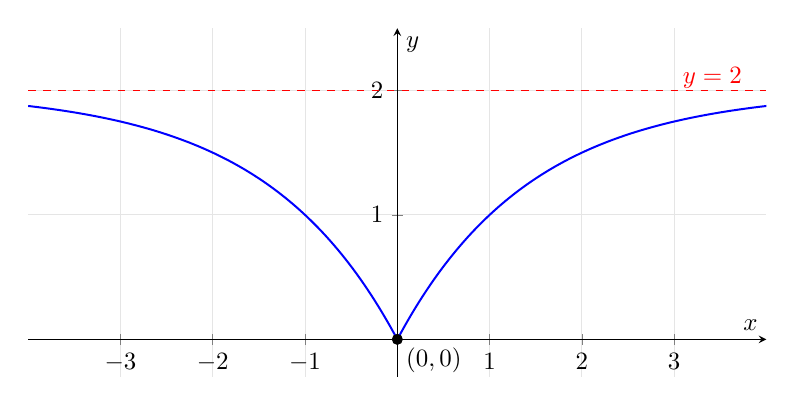
\begin{tikzpicture}[scale=0.9]
\begin{axis}[
    width=12cm, height=6.5cm,
    axis lines=middle,
    xlabel=$x$, ylabel=$y$,
    xmin=-4, xmax=4, ymin=-0.3, ymax=2.5,
    xtick={-3,-2,-1,0,1,2,3},
    ytick={1,2},
    grid=major, grid style={gray!20},
]
\addplot[thick,blue,domain=0:4,samples=100] {2-2*0.5^x};
\addplot[thick,blue,domain=-4:0,samples=100] {2-2*0.5^(-x)};
\draw[dashed,red] (axis cs:-4,2)--(axis cs:4,2);
\node[red,right] at (axis cs:3,2.1) {$y=2$};
\addplot[only marks,mark=*,mark size=2pt,black] coordinates {(0,0)};
\node[below right] at (axis cs:0,0) {$(0,0)$};
\end{axis}
\end{tikzpicture}
\end{center}
\end{frame}

\begin{frame}[t]{第9题 解答：(2)}
\begin{tcolorbox}[colback=orange!10,colframe=orange,title=\textbf{解：(2)}]
\textbf{奇偶性：} 对任意 $x\in\mathbf{R}$，
\[
f(-x)=2-2\left(\frac12\right)^{|-x|}=2-2\left(\frac12\right)^{|x|}=f(x),
\]
故该函数为\alert{偶函数}，图象关于 $y$ 轴对称。

\vspace{0.6em}
\textbf{单调性：}
\begin{itemize}
  \item 当 $x\ge 0$ 时，$y=2-2\cdot\left(\frac12\right)^{x}$，因为 $\left(\frac12\right)^{x}$ 递减，所以 $y$ 在 $[0,+\infty)$ 上\alert{单调递增}；
  \item 由偶函数图象关于 $y$ 轴对称，$y$ 在 $(-\infty,0]$ 上\alert{单调递减}。
\end{itemize}
\end{tcolorbox}
\end{frame}

% ========== 第10题 ==========
\begin{frame}[t]{第10题：两个指数函数的比较}
\textbf{10.} 已知 $f(x)=a^{x},\ g(x)=\left(\dfrac{1}{a}\right)^{x}\ (a>0,\ \text{且 }a\ne 1)$。

(1) 讨论函数 $f(x)$ 和 $g(x)$ 的单调性；

(2) 如果 $f(x)<g(x)$，那么 $x$ 的取值范围是多少？
\end{frame}

\begin{frame}[t]{第10题 解答}
\begin{tcolorbox}[colback=orange!10,colframe=orange,title=\textbf{解}]
\textbf{(1)} 因为 $\left(\frac1a\right)^{x}=a^{-x}$：
\begin{itemize}
  \item 当 $a>1$ 时，$y=a^{x}$ 是增函数，$y=\left(\frac1a\right)^{x}=a^{-x}$ 是减函数；
  \item 当 $0<a<1$ 时，$y=a^{x}$ 是减函数，$y=\left(\frac1a\right)^{x}=a^{-x}$ 是增函数。
\end{itemize}
即两者单调性始终相反。

\vspace{0.6em}
\textbf{(2)} 由 $f(x)<g(x)$：
\[
a^{x}<\left(\frac1a\right)^{x}=a^{-x}.
\]
\begin{itemize}
  \item 若 $a>1$，$y=a^{x}$ 递增，故 $x<-x$，即 $\alert{x<0}$；
  \item 若 $0<a<1$，$y=a^{x}$ 递减，故 $x>-x$，即 $\alert{x>0}$。
\end{itemize}
\end{tcolorbox}
\end{frame}

\begin{frame}[t]{第10题 图象示意}
	\vspace{2em}
\begin{center}
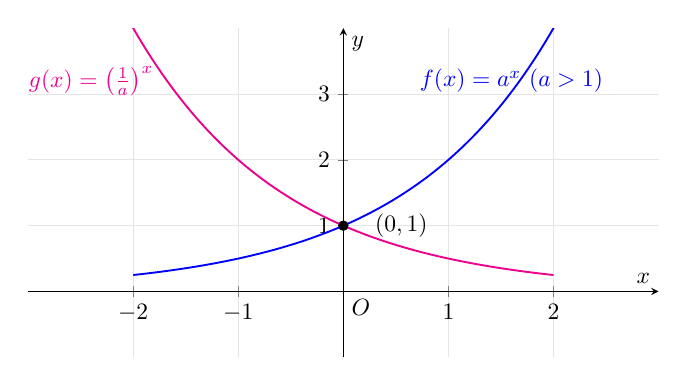
\begin{tikzpicture}[scale=0.85]
\begin{axis}[
    width=11cm, height=6.5cm,
    axis lines=middle,
    xlabel=$x$, ylabel=$y$,
    xmin=-3, xmax=3, ymin=-1, ymax=4,
    xtick={-2,-1,0,1,2},
    ytick={1,2,3},
    grid=major, grid style={gray!20},
]
\addplot[thick,blue,domain=-2:2.5,samples=100] {2^x};
\addplot[thick,magenta,domain=-2.5:2,samples=100] {0.5^x};
\node[blue] at (axis cs:1.6,3.2) {$f(x)=a^{x}\ (a>1)$};
\node[magenta] at (axis cs:-2.4,3.2) {$g(x)=\left(\frac1a\right)^{x}$};
\addplot[only marks,mark=*,mark size=2pt,black] coordinates {(0,1)};
\node[right=1em] at (axis cs:0,1) {$(0,1)$};
\node[below right] at (axis cs:0,0) {$O$};
\end{axis}
\end{tikzpicture}
\end{center}
\end{frame}

\begin{frame}[c]
  \begin{center}
    {\Huge\calligra Thanks!}
  \end{center}
\end{frame}

\end{document}
